\documentclass[addpoints, 12pt] {exam}
\usepackage{graphicx}
\usepackage{amsmath}
\bracketedpoints
\pagestyle{headandfoot}
\runningheadrule
\firstpageheader{Math 112}{Written Homework 1}{Due January 19th, 2024}
\runningheader{Math 112}{ Page\; \thepage\; of\; \numpages}{Written Homework 1}
\firstpagefooter{}{}{}
\runningfooter{}{}{}
\setlength\answerskip{2ex}
\setlength\answerlinelength{1.5in}
\begin{document}

\begin{center}
\fbox{\fbox{\parbox{5.5in}{\centering
Directions:\\Please only put your final, well written solutions, in the space provided.\\ Give exact answers (simplified radicals or fractions).\\If you use additional paper clearly label the question and upload pages after the question page.\\Use complete sentences and explain your reason as much as possible.\\There are \numquestions\,  questions and \numpoints\, points total
}}}\end{center}
\vspace{0.1in}
\makebox[\textwidth]{Name:\enspace\hrulefill}
%\qformat{Question \thequestion \dotfill \thepoints}%

Before you begin this assignment, I would like to emphasize one of the \textbf{most important} concepts/definitions for this entire course: 
\begin{center}
\emph{What (mathematically) is a function?}
\end{center}
\textbf{Definition of a Function:} 
\begin{center}
We say that \(y\) (the output variable) is a \textbf{function} of \(x\) (the input variable) when the following is true:

 \emph{\textbf{For any given input \(x\), there is one and only one output \(y\).}}
\vspace{0.5in}

\end{center}
A known consequence of this definition is that, when graphed with the output as the vertical axis and the input as the horizontal axis, the graph will ``pass'' the vertical line test, e.g., any vertical line drawn on the same coordinate system will only intersect the the graph once. This is known as the \textbf{vertical line test} and can be used to justify that something is a function.
\vspace{0.25in}

Please refer to this page whenever you are asked to consider whether or not something is a function.\newpage
\begin{questions}

\question Consider the following situation: Universities around the world charge tuition to their students each semester. Typically, there are tuition price increases every year. We will consider a simplified version of this where we shall suppose the following: Beginning in 2023, the tuition at a particular school is \(\$20,000\) per year and every year the university plans to increase this tuition by a fixed \(3.75\%\) of the 2023 tuition (the tuition increase will be the exact same each year).
\begin{parts}
\part[1] \textbf{Why} does this description express tuition as a function of cost per year since 2023 (recall: what is the definition of a function)? You may define your own input/output variables. \vspace{1.75in}
\part[5] Write the mathematical definition for this function. Use \(C\) as the output function name and \(t\) as the input of time, in years, since 2023. Put your answer on the answerline, but show your final, cleanly written work in the space provided.\vspace{0.75in}\answerline
\part[2] What is a reasonable domain for this function? Put your answer on the line provided using interval notation.\vspace{0.25in}\answerline
\part[2] Using the function you created, in what year will the tuition exceed \(\$50,000\)? Please show your calculation steps in the space provided. If you use a graphing calculator, state what you did to solve the question. \vspace{0.5in}\answerline
\end{parts}\newpage
\question The area of a triangle is given by the formula: \[A=\frac{1}{2}bh\]where \(b\) is the length of the base of the triangle and \(h\) is the length of the height of the triangle.  The height and the base must be perpendicular to each other.
\begin{parts}
\part[3] Draw a picture representing this description. There are *many* correct ways to draw this and you are welcome to look up information about this. However, please make your own drawing easy to view, large and well-labeled.\vspace{2.5in}
\part[5] Suppose that the height of the triangle is \(10cm\) \textbf{more than} the base of the triangle. Using the formula provided, what is the equation for the area of this triangle?  Your answer will have \(b\) and \(A\) in it. \vspace{1in} \answerline
\part[2] Use your formula in the previous part to determine the area of the triangle if the base is \(42cm\). Show all your final work in the space provided. \vspace{1in}\answerline
\end{parts}
\newpage
\question Consider the following table which relates the demand of coffee for different prices.
\[
\begin{array}{|l|c|c|c|c|c|}
\hline
\text{Price(\$)}&1.25&0.75&2.5&2.5\\\hline
\text{Demand(Units)}&500&1000&425&375\\
\hline
\end{array}
\]
\begin{parts}
\part[2]In the space provided, create a plot where the {\bf horizontal} axis is {\bf demand} and the {\bf vertical} axis is {\bf price}. Make sure every combination of values from the table is included. Do {\bf not} connect the dots (this table only defines the pairs as given). Label each axis and the scale of each axis (indicate what you are counting by on each axis).\vspace{2in}
\part[3]Explain whether or not {\bf Price} is a function of {\bf Demand}.\vspace{1in}
\part[2]In the space provided, create a plot where the {\bf horizontal} axis is {\bf price} and the {\bf vertical} axis is {\bf demand}. Do the rest the same as you did the first part.\vspace{2in}
\part[3]Explain whether or not {\bf Demand} is a function of {\bf Price}.\vspace{1in}
\end{parts}
\newpage
\question Use the graph to answer the questions:\newline
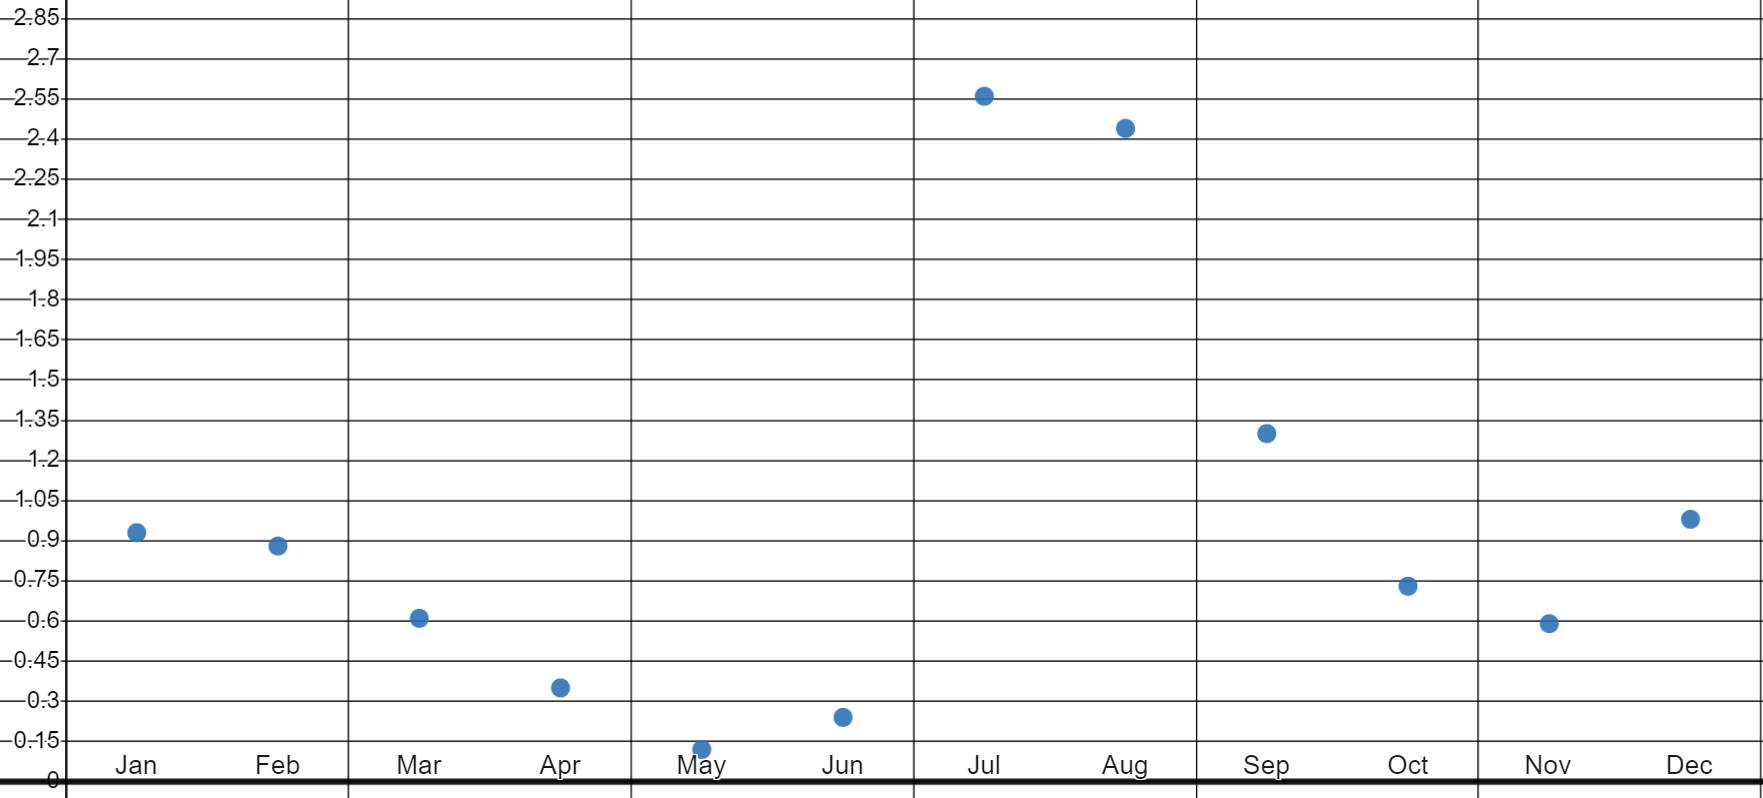
\includegraphics[scale=0.35]{TucsonRainData}\newline
The vertical axis represents the number of {\bf inches} of rain that Tucson experiences {\bf on average} for each particular month (the horizontal axis).
\begin{parts}
\part[2]In your own words, describe what constitutes the {\bf domain} of this graph.\vspace{0.5in}
\part[2]In your own words, describe what the (approximate) range of this graph is. \vspace{0.5in}
\part[3]In your own words, provide an interpretation of the graph. Note features that stand out to you. Try to incorporate correct mathematical language in your response. \vspace{1in}
\part[3]Consider a hypothetical situation: if you were given data for a particular month that indicated the amount of rain Tucson had received, but the month was redacted, could you determine the month with the information you have on hand? Provide an {\bf argument} and justify your position. There is no `right` or `wrong` answer as long as you argue your point and justify your conclusion. 
\end{parts}
\end{questions}


\end{document}